\documentclass[a4paper]{article}


\usepackage{alphabeta} 
\usepackage{enumitem} 
\usepackage{mathtools}
\usepackage{amsmath, amssymb} 
\usepackage{amsthm}
\usepackage{cancel} 
\usepackage[margin=0.70in]{geometry} 
\geometry{left=2.9cm,right=3.0cm,top=2.1cm,bottom=2.3cm}	%the page geometry as defined, A4=210x297mm
\usepackage{graphicx}
\usepackage{wrapfig}
\usepackage{caption}
\usepackage{textcomp}
\usepackage{tabto}
\usepackage{layout}
\usepackage{bm}
\usepackage{minipage-marginpar}
\usepackage[dvipsnames]{xcolor}
\usepackage{hyperref}
\usepackage{dutchcal}
\usepackage{derivative}
\usepackage{esint}
%\usepackage{biblatex}
\usepackage{subcaption}
\usepackage{booktabs}\usepackage{derivative}
\usepackage[flushleft]{threeparttable}
\usepackage[capbesideposition=outside,capbesidesep=quad]{floatrow}
\usepackage{derivative}
\usepackage[thinc]{esdiff}
%%RENEW

\newtheorem{problem}{Άσκηση}
\newtheorem*{solution*}{Λύση}
\newtheorem{definition}{Ορισμός}[subsection]
\newtheorem{properties}{Ιδιότητες}[subsection]
\newtheorem{theorem}{Θεώρημα}[subsection]
\newtheorem{protash}{Πρόταση}[subsection]
\newtheorem{porisma}{Πόρισμα}[subsection]
\newtheorem{lemma}{Λήμμα}[subsection]
\newtheorem*{prooof}{Απόδειξη}
\newtheorem*{notes}{Παρατηρήσεις}
\newtheorem*{note}{Παρατήρηση}
\newtheorem*{app}{Εφαρμογή} 
\newtheorem*{example}{Παράδειγμα}
\newtheorem*{examples}{Παραδείγματα}


\newcommand\numberthis{\addtocounter{equation}{1}\tag{\theequation}}
%\renewcommand{\labelenumi}{\roman{enumi}}
\newcommand{\approxtext}[1]{\ensuremath{\stackrel{\text{#1}}{\approx}}}
\renewcommand{\figurename}{Εικόνα.}
\renewcommand{\tablename}{Πίνακας.}
%\renewcommand\refname{New References Header}
\renewcommand*\contentsname{Περιεχόμενα}
%\DeclareDerivative{\odv}{\mathrm{d}}


\begin{document}
\begin{titlepage}			%makes a title page. Remember to change the author, CID, username and group number to what is appropriate for you!
	\centering
	{\scshape\LARGE Εθνικό Μετσόβιο Πολυτεχνείο\par}
	{\scshape \LARGE Σ.Ε.Μ.Φ.Ε.\par}
	\vspace{1cm}
	{\huge\bfseries Μέτρηση του Συντελεστή Θερμικής Αγωγιμότητας Υλικών \par}
	\vspace{1cm}
	{\Large\itshape Θωμόπουλος Σπύρος\par}		%remember to change these!
	
	%		{\large Group \@group\unskip\strut\par}
	{\large A.M  \hfill \\ E-mail spyros.thomop@gmail.com \\}%ge19042@mail.ntua.gr\par		%remember to change these!
	\vspace{1cm}
	{\large Ημερμονηνία Παράδοσης 15/12/2021\par}
\end{titlepage}


\newpage 

\subsection*{Σκοπός}

Ο στόχος της εν λόγω πειραματικής άσκησης είναι ο προσδιορισμός του συντελεστή θερμικής αγωγιμότητας δύο υλικών, ενός αγωγού και ενός μονωτή. Επιπλέον, θα προσδιορίσουμε τον χρόνο θέρμανσης μίας μεταλλικής ράβδου και την κατανομή της θερμοκρασίας κατά το μήκος της.

\subsection*{Θεωρητικά Στοιχεία}

Σε μεγάλο μέρος της άσκησης αυτής θα μελετηθεί μία ράβδος από ορείχαλκο. Όταν η ράβδος διατηρεί αμετάβλητες τις ιδιότητές της (θερμοδυναμικές μεταβλητές) για σταθερές εξωτερικές συνθήκες λέμε ότι βρίσκεται σε κατάσταση ισορροπίας και αντιθέτως, αν μεταβάλλονται, τότε είναι εκτός ισορροπίας και εμφανίζονται \textit{φαινόμενα μεταφοράς} και συγκεκριμένα \textit{θερμικής αγωγιμότητας.} Στο προαναφερθέν παράδειγμα της ράβδου τέτοιου είδους φαινόμενα θα εμφανίζονται όταν η ροή θερμότητας κατά μήκος της δεν είναι ίδια σε όλα τα σημεία.

Μαρκοσκοπικά, θα έχουμε ροή θερμότητας από τα θερμά στα ψυχρά σημεία με αποτέλεσμα την σταθεροποίηση της θερμοκρασίας κάθε σημείου σε κάποιον χαρακτηριστικό χρόνο, ενώ σε μικροσκοπικό επίπεδο έχουμε περιοχές με πιό έντονες θερμικές ταλαντώσεις των μορίων, η ενέργεια των οποίων μεταφέρεται στις περιοχές με πιό ασθενεις ταλαντώσεις εως ότου η ροή ενέργειας εξισοροπιστεί. 
Επιπλέον, στα μέταλλα υπάρχει και η καθοριστική συνεισφορά των ελεύθερων ηλεκτρονίων που μπορούν να μεταφέρουν την ενέργεια με πιο αποδοτικό τρόπο. Πρακτικά, εμείς μπορούμε να προσδιορίσουμε το πόσο 'καλό' ή 'κακό' είναι ένα υλικό στο να άγει την θερμότητα από το εσωτερικό του με τον προσδιορισμό του συντελεστή θερμικής αγωγιμότητας.

\subsubsection*{Αγωγοί}
Αν έχουμε μία μεταλλική ράβδο η οποία δεν βρίσκεται σε θερμική ισορροπία, τότε για ένα δεδομένο χρονικό διάστημα dt, η θερμότητα που ρέει από μία διατομή της εμβαδού S προς μία άλλη, η οποία απέχει κατά dx χωρικά και κατά dT θερμοκρασιακά θα είναι
\begin{align*}\label{1}
\frac{dQ}{dt} \propto S\frac{dT}{dx} \numberthis
\end{align*}
ο συντελεστής αναλογίας των δύο ποσοτήτων είναι στθερός για κάθε υλικό ανεξάρτητα του αν είναι διαμορφωμένο σε σχήμα ράβδου και πρόκειται για τον \textit{συντελεστή θερμικής αγωγιμότητας, λ}. Όσο πιο μεγάλος είναι τόσο πιο αγώγιμο είναι το υλικό στο οποίο αναφέρεται. Ακόμη στην σχέση (\ref{1}) θα πρέπει να προσθέσουμε ένα "-" το οποίο θα δηλώνει το γεγονός ότι η θερμότητα ρέει από τις θερμές στις ψυχρές περιοχές της ράβδου.

Για πεπερασμένες μεταβολές των μεγθών της σχέσης (\ref{1}) τις οποίες μπορούμε να μετρήσουμε/επιβάλλουμε πειραματικά και παρατηρώντας ότι το αριστερό μέλος πρόκειται για ισχύ παίρνουμε την σχέση
\begin{align*}\label{2}
P = \frac{\Delta Q}{\Delta t} = - \lambda S \frac{\Delta T}{\Delta x} \xRightarrow[\Delta x=L]{\text{Όλη η ράβδος}}  
				\frac{\Delta T}{L} = -\frac{1}{\lambda S} P \numberthis
\end{align*}
Άρα επιβάλλοντας μία σταθερή ισχύ στο ένα άκρο και μετρώντας την θερμοκρασική διαφορά των δύο άκρων μπορούμε με μία μέθοδο ελαχίστων τετραγώνων να προσδιορίσουμε τον συντελεστή λ ($[\lambda]=[W\cdot K^{-1}\cdot m^{-1}])$.
\\
Πέρα από την μεταφορά της θερμότητας, μας ενδιαφέρει και η κατανομή της θερμοκρασίας κατά μήκος της ράβδου. Η εν λόγω κατανομή μπορεί να προκύψει ως λυση της διαφορικής εξίσωσης 
\begin{align*}\label{3}
\rho c \pdv{T}{t} = \lambda\pdv[2]{T}{x}  \numberthis
\end{align*}

όπου ρ η πυκνότητα και c η ειδική θερμότητα του υλικού.
Στο πείραμα επιβάλλουμε ως συνοριακές συνθήκες της εξίσωσης (\ref{3}) για το ένα άκρο να θερμαίνεται σε σταθερή θερμοκρασία $T_L$ και για το άλλο να βρίσκεται σε θερμοκρασία περιβάλλοντος $T_\pi$. 
 

Όταν επέλθει η θερμική ισορροπία της ράβδου, ($dQ/dt=$σταθ. από κάθε διατομή της και Τ ανεξάρτητη του χρόνου για κάθε σημείο της) τότε η θερμοκρασιακή κατανομή θα είναι γραμμική
\begin{align*}\label{4}
T(x) = T_\pi +\frac{T_L-T_\pi}{L}x \numberthis
\end{align*}
Ο χρόνος $\tau_0$ που απαιτείται για την ισορροπία έχει έντονη εξάρτηση από το μήκος της ράβδου ενώ δεν εξαρτάται από την διατομή της: 
\begin{align*}\label{5}
\tau_0 \sim \rho c L^2 /\lambda \numberthis
\end{align*}

\textcolor{red}{Ακόμη, έχουμε ότι η θερμοκρασία του θερμαινόμενου άκρου αυξάνεται εκθετικά μέχρι να φτάσει την τιμή $T_L$.}

\subsubsection*{Μονωτές}

Εδώ θα μελετηθεί ένα φύλλο από θερμομονωτικό υλικό. Όταν το τοποθετήσουμε ενδιάμεσα σε ένα σώμα μεγάλης θερμοχωρητικότητας και σε έναν θερμό μεταλλικό δίσκό, τότε ο δίσκος θα πρέπει να χάνει θερμότητα γρηγορότερα απ' ότι θα έχανε αν ήταν σε επαφή π.χ. μόνο με το περιβάλλον. Αν m  η μάζα του και c η ειδική του θερμότητα, τότε την χρονική στιγμή t και βρισκόμενος σε θερμοκρασία T θα έχει χάσει θερμότητα:
\begin{align*} \label{6}
Q=mc(T-T_\pi) \Rightarrow \odv{Q}{t}=mc\odv{(T-T_\pi)}{t} \numberthis
\end{align*}

Αν λάβουμε υπόψιν μας και το ότι η θερμότητα που ρέει απ' τον φύλλο δίνεται από την (\ref{1}) και ισούται με αυτήν που χάνεται απ' τον δίσκο (οι απώλειες προς το περιβάλλον είναι πολύ μικρότερες), τότε καταλήγουμε στην σχέση 
\begin{align*}\label{7}
T = T_\pi + (T_0 - T_\pi )e^{-\frac{\lambda S}{mca}t} \numberthis
\end{align*}
όπου α το παχος του λεπτού φύλλου και S το εμβαδό του δίσκου. Δηλαδή η θερμοκρασία του δίσκου μειώνεται εκθετικά με την παρεμβολή του λεπτού μονωτικού φύλλου.

\subsection*{Πειραματική Διάταξη}
Η πειραματική διάταξη αποτελείται από: 
\begin{itemize}
\item[$\rightarrow$] \underline{\textbf{Αγωγοί}}
	\begin{itemize}
		\item[.] Μεταλλική Ράβδο από ορείχαλκο διαμέτρου $d_1 = (11.0\pm0.1)mm$, μήκους $L=(70.0\pm0.1)mm$ η οποία έχει ανά 									$(15.0\pm0.1)mm$ 5 εσοχές.
		\item[.] Τροφοδοτικό που μέσω ηλεκτρικού λαμπτήρα παρέχει στο άκρο της ράβδου σταθερή ισχύ που κυμαίνεται από $0-15W$
				\item[.] Ψηφιακό θερμόμετρο για μέτρηση της θερμοκρασίας στις 5 εσοχές της ράβδου
		\item[.] Χρονόμετρο
		\end{itemize}
\item[$\rightarrow$] \underline{\textbf{Μονωτές}} 
	\begin{itemize}
		\item[.] Μεταλλικό δίσκο διαμέτρου $d_2 = (59.0\pm0.3)mmm$ με δύο υποδοχές, μία για θερμόμετρο και μία για τον θερμαντήρα
		\item[.] Μονωτικό φύλλο πάχους $a=(0.100\pm0.005)mm$
		\item[.] Ηλεκτρικός θερμαντήρας
		\item[.] Χρονόμετρο
	\end{itemize}
\end{itemize}
Στα δύο μέρη του πειράματος χρησιμοποιείται ως σώμα μεγάλης θερμοχωρητικότητας ένα σώμα μάζας 15kg. Τα κύρια μέρη της διάταξης φαίνονται στην Εικόνα 1. 
\begin{figure}[h!]
\centering
\caption{ Πειραματική Διάταξη}
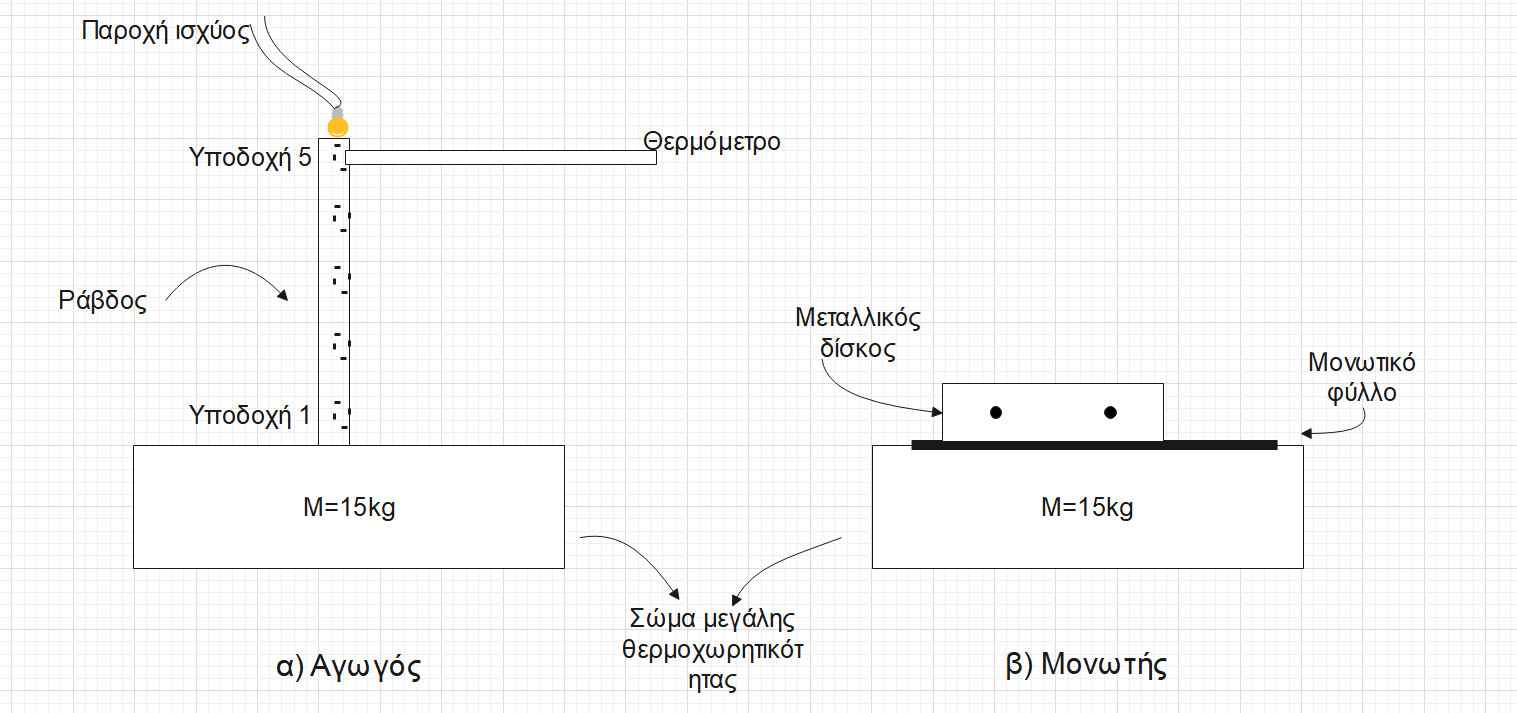
\includegraphics[scale=0.285]{setup.png}
\end{figure}


\subsection*{Πειραματική Διαδικασία - Επεξεργασία Μετρήσεων}

\subsubsection*{Στθερά χρόνου θέρμασης $\tau_0$}
Αρχικά τοποθετούμε το θερμόμετρο στην υποδοχή του σώματος μεγάλης θερμοχωρητικότητας και έτσι μετράμε την θερμοκρασία του περιβάλλοντος $T_{\pi\epsilon\rho.1} = (18.8\pm0.5)^oC$ και στη συνέχεια θέτουμε το τροφοδοτικό σε λειτουργία στα $P=(3.0\pm0.5)W$. Τώρα μετράμε την θερμοκρασία σε αυτή την υποδοχή ανά $30sec$ για τα επόμενα $5min$. Τα αποτελέσματα φαίνονται στον Πίνακα Ι.
\begin{table}[h!]
\begin{tabular}{r|r}
\centering
\caption{ }
$t(\pm1 s)$ & $T_5(\pm0.5 ^oC)$ \\ 
\hline\hline
0&18.8\\
30&21.4\\
60&23.7\\
90&25.4\\
120&26.5\\
150&27.3\\
180&27.9\\
210&28.3\\
240&28.6\\
270&28.7\\
300&28.8\\
\end{tabular}
\end{table}

Η γραφική παράσταση των παραπάνω μεγεθών φαίνεται στην Εικόνα 2.
\begin{figure}[h!]
\centering
\caption{ $T=T(t)$, υποδοχή 5}
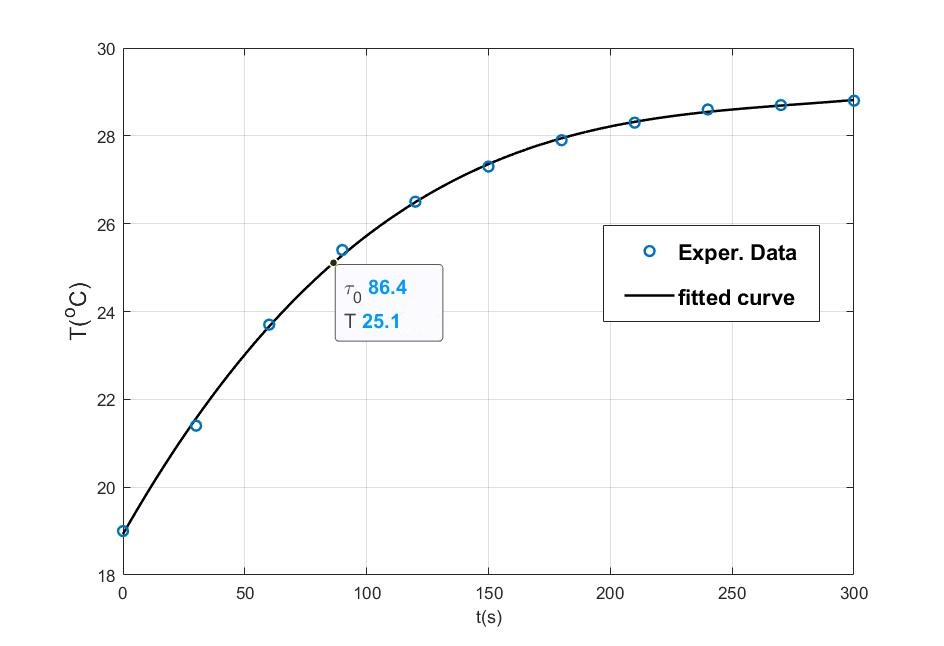
\includegraphics[scale=0.7]{t0.jpg}
\end{figure}

Στον χρόνο θέρμανσης, $\tau_0$, η θερμοκρασία φτάνει στο $63\%$ της μέγιστης μεταβολής της, άρα σε θερμοκρασία  
$T(\tau_0) =T_{περ}+  0.63\Delta T_{max} = 18.8 + 0.63\cdot 10^oC = 25.1^oC$. \textcolor{red}{Άρα η σταθερά χρόνου θέρμανσης της ράβδου είναι $\tau_0 = 86sec$.}        %palia 85

Από την σχέση (\ref{5}) έχουμε 
\begin{align*}
\frac{\tau_{0}(L=7cm)}{\tau_0(L'=49cm)} =\frac{L^2}{L'^2} = \frac{1}{49} \Rightarrow \tau_0'(L'=49cm) = 49\cdot \tau_{0}(L=7cm) = 4214sec
\end{align*}
H μεταβατική περίοδος θα διαρκεί περίπου $t_{\text{μεταβ'}} \simeq 5 \tau_0' = 21071sec \simeq 351 min$ για την ράβδο μεγάλου μήκους 49cm και για την μικρή ράβδο που θα μελετηθεί είναι $t_{\text{μεταβ}} \simeq 5\tau_0 = 430sec \simeq 7min.$

\subsubsection*{Μέτρηση συντελεστή θερμικής αγωγιμότητας $\lambda$ της ράβδου}
Τώρα που ξέρουμε τον μεταβατικό χρόνο που απαιτείται για να έρθει σε ισορροπία το σύστημα, δηλαδή πρακτικά το διάστημα που πρέπει να περιμένουμε μετά από μία αλλαγή σε συνοριακή συνθήκη (εφαρμοζόμενη ισχύς) ώστε να πάρουμε μία μέτρηση σε ισορροπία, μπορούμε να προσδιορίσουμε τον συντελεστή λ.

Ξεκινώντας από ισχύ $P=3-15W$ με βήμα $3W$ καταγράφουμε την θερμοκρασία στις ακριανές υποδοχές 1 και 5. Σε κάθε αλλαγή περιμένουμε $5-7min$ ώστε να επέλθει η θερμική ισορροπία. Οι δύο ακραίες εγκοπές απέχουν $L_{1-5} = (6.00\pm0.02)cm$. Τα αποτελέσματα φαίνονται στον Πίνακα 2. 
\begin{table}[h!]
\centering
\caption{ }
\begin{tabular}{r|r|r|r}
$P(\pm0.5W)$ & $T_1(\pm0.5^oC)$ & $T_5(\pm0.5^oC)$ & $(T_5-T_1)/L_{1-5}(^oC/m)$\\ 
\hline\hline
3.0&28.8&20.1  &145.0\\
 6.0&41.1&22.4  &311.7\\
 9.0&51.4&23.4  &466.7\\
12.0&64.8&25.5  &655.0\\
15.0&73.0&27.1  &765.0
\end{tabular}
\end{table}

To μέγεθος $\Delta T /\Delta x$ που εμφανίζεται στην τελευταία στήλη καλείται θερμοβαθμίδα και η γραφική του παράσταση συναρτήσει της ισχύος είναι:

\begin{figure}[h!]
\centering
\caption{ Θερμαβαθμίδα $\Delta T/\Delta x$ - Ισχύς }
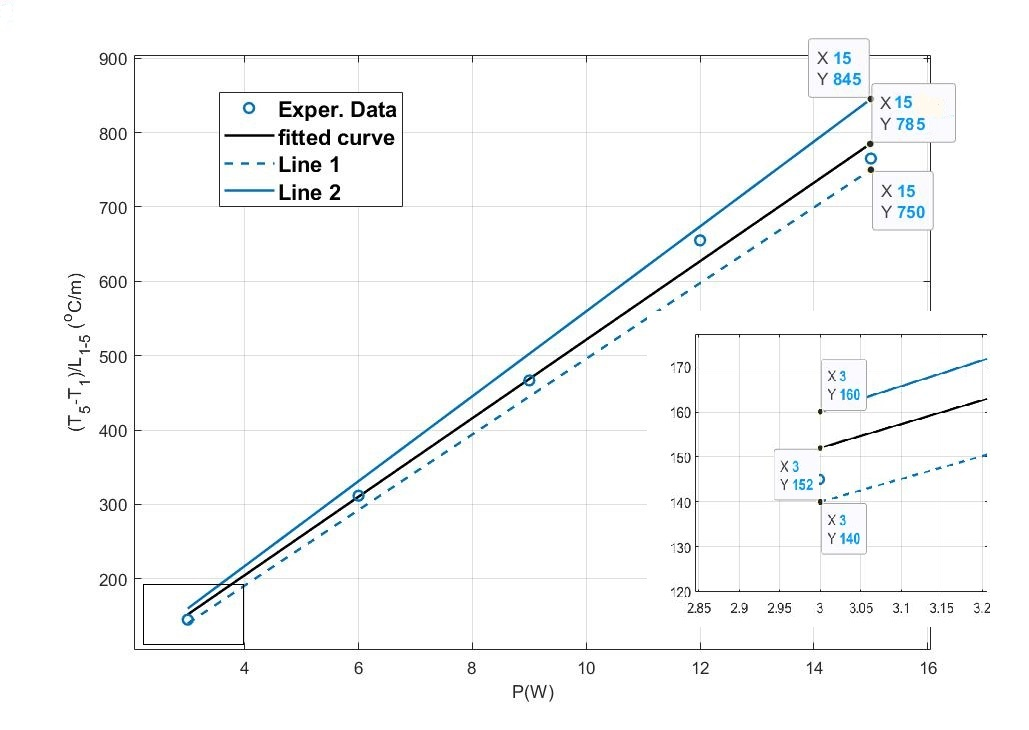
\includegraphics[scale=0.8]{pDxDt.jpg}
\end{figure}



Η κλίση Β της βέλτιστης ευθείας, όπως προκύπτει από την παραπάνω γραφική παράσταση είναι 
\begin{align*}
B=\frac{785-152}{15-3} \simeq 53
\end{align*}
Αντίστοιχα, οι κλίσεις των ευθειών 1 και 2 είναι 
\begin{align*}
B_1 = \frac{750-140}{15-3} \simeq 51  \textbf{ και }
B_2 = \frac{845-160}{15-3} \simeq 57
\end{align*}
Το σφάλμα της κλίσης της βέλτιστης ευθείας είναι 
\begin{align*}
\delta B = 0.5(B_2-B_1) = 3
\end{align*}
Άρα έχουμε ότι: $B = (53\pm3) [S.I.]$.
Επομένως, αν εκμεταλλευτούμε την (\ref{2}) με δεδομένο ότι το εμβαδό της διατομής της ράβδου είναι $S=(95.0\pm17.3)mm^2$  \footnotemark, προκύπτει ότι η κλίση Β ισούται με 
\footnotetext{$S=\pi(d_1/2)^2=95.0mm^2$ με σφάλμα από την διάδοση του σφάλματος της διαμέτρου $\delta S = |\pdv{S}{d_1}\delta d_1|=\pi d_1/2\simeq 17.3mm^2$}
\begin{align*}
B = \frac{1}{\lambda S} \Rightarrow \lambda =\frac{1}{BS} = 198.809\simeq199   [S.I.]
\end{align*}
Το σφάλμα προκύπτει από την διάδοση των σφαλμάτων των S, B:
\begin{align*}
\delta \lambda=\sqrt{\left( \pdv{\lambda}{B}\delta B \right)^2+\left( \pdv{\lambda}{S}\delta S\right)^2} = \frac{1}{SB}
\sqrt{\left( \frac{1}{B}\delta B\right)^2+\left( \frac{1}{S}\delta S \right)^2} \simeq 38  [S.I]
\end{align*}
Άρα έχουμε ότι $\boxed{\lambda_{\text{ορειχ}}=(199\pm38)Wm^{-1}K^{-1}}$

Τώρα παρέχοντας στο άκρο ισχύ 15W μετράμε την θερμοκρασία σε όλες τις υποδοχές τις ράβδου: 
Από τον Πίνακα 3 προκύπτει και η γραφική πραάσταση, η οποία προφανώς αναφέρεται στη μόνιμη κατάσταση της ράβδου που φαίνεται στην Εικόνα 4.


\begin{table}[h!]
\centering
\caption{ }
\begin{tabular}{r|r}
$x(cm)\footnotemark$ & $T(^oC)$ \\
\hline\hline
0.5&27.1\\
2.0&38.0\\
3.5&47.8\\
5.0&61.3\\
6.5&73.3
\end{tabular}
\end{table}
\footnotetext{Το x ξεκινά από 0.5cm διότι η υποδοχή 1 δεν ακουμπά στο σώμα μεγάλης θερμοχωρητικότητας αλλά απέχει από αυτό 5cm. }


\begin{figure}[h!]
\centering
\caption{ Κατανομή θερμοκρασίας στην μόνιμη κατάσταση}
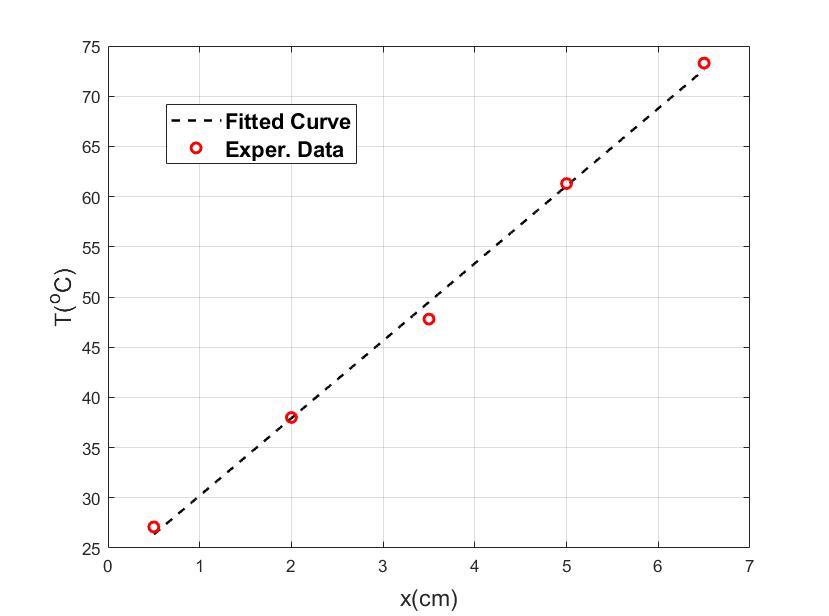
\includegraphics[scale=0.53]{Tdistr.jpg}
\end{figure}


\subsubsection*{Μέτρηση του συντελεστή θερμικής αγωγιμότητας του μονωτικού φύλλου}

Αρχικά, πρέπει να προσδιορίσουμε την μάζα του μεταλλικού δίσκου που θα μελετηθεί. Ζυγίζοντάς τον προκύπτει ότι $m=(350.6\pm0.1)gr$. Τοποθετούμε τον δίσκο σε μία μονωτική βάση προκειμένου να μελετήσουμε την απώλεια θερμότητάς του προς το περιβάλλον. 

Τοποθετούμε το θερμόμετρο στην ρηχή εσοχή του και τον ηλεκτρικό θερμαντήρα στην πιό βαθιά. Τώρα θερμαίνουμε τον δίσκο μέχρι να φτάσει σε θερμοκρασία $75^oC$.
Με το θερμόμετρο μετράμε για τα επόμενα $3min$ και ανά $30sec$ την θερμοκρασία του δίσκου. Οι μετρήσεις φαίνονται στον Πίνακα 4. 
\begin{table}[h!]
\centering
\caption{Δίσκος-Περιβάλλον }
\begin{tabular}{r|r}
$t(s\pm1)$ & $T(\pm0.5 ^oC)$ \\ 
\hline\hline
0&75.1\\
30&74.1\\
60&73.1\\
90&72.2\\
120&71.3\\
150&70.3\\
180&69.7\\
210&68.5\\
240&67.7\\
270&66.8\\
300&65.9
\end{tabular}
\end{table}

Στην συνέχεια, προκειμένου να μελετήσουμε την μεταβολή της θερμοκρασίας του δίσκου κατά την επαφή του με τον μονωτή, τοποθετούμε τον μεταλλικό δίσκο επί του μονωτικού φύλλου το οποίο έχουμε ακουμπήσει στην επιφάνεια του σώματος μεγάλης θερμοχωρητικότητας. Mετράμε την θερμοκρασία του δίσκου για τα επόμενα 6min με βήμα 30sec. Τα αποτελέσματα φαίνονται στον Πίνακα 5.
Ακόμη, στο τέλος τοποθετούμε το θερμόμετρο στην εσοχή του σώματος μεγάλης θερμοχωρητικότητας για να ξαναμετρήσουμε την θερμοκρασία του περιβάλλοντος: $T_{\pi\epsilon\rho,2}=(21.1\pm0.5)^oC$ και βλέπουμε ότι έχει αθξηθεί από την αρχική μέτρηση (ενδεχομένως εξαιτίας της πρόσπτωσης των ηλιακών ακτίνων καθώς και της παρουσίας μας στον χώρο του εργαστηρίου).
\begin{table}[h!]
\centering
\caption{ Δίσκος-Μονωτής}
\begin{tabular}{r|r|r}
$t(\pm1s)$ & $T(\pm0.5^oC)$ & $ln(T-T_{\pi\epsilon\rho,2})$  \\ 
\hline\hline
0&64.0&3.759\\
30&59.4&3.645\\
60&55.3&3.532\\
90&51.7&3.421\\
120&48.5&3.311\\
150&45.7&3.203\\
180&43.2&3.096\\
210&41.0&2.994\\
240&39.0&2.885\\
270&37.2&2.779\\
300&35.5&2.667\\
330&34.2&2.573\\
360&32.9&2.468
\end{tabular}
\end{table}


Από τα δεδομένα των Πινάκων 4 και 5 προκύπτει η γραφική παράσταση (Εικόνα 5.) της μεταβολής της θερμοκρασίας του δίσκου όταν αυτός βρίσκεται επί της μονωτικής βάσης (απώλεια προς το περιβάλλον) και όταν είναι επί του μονωτικού φύλλου (απώλεια εξ'αιτίας του φύλλου). 

Παρατηρούμε ότι η απώλεια θερμότητας, απόρροια της οποίας είναι η μέιωση της θερμοκρασίας του δίσκου, γίνεται πιό γρήγορα (θεωρητικά εκθετικά) όταν τον τοποθετούμε στο μονωτικό φύλλο.

\newpage

\begin{figure}[h!]
\centering 
\caption{ Απώλεια θερμότητας του δίκου προς περιβάλλον / μονωτικό φύλλο.}
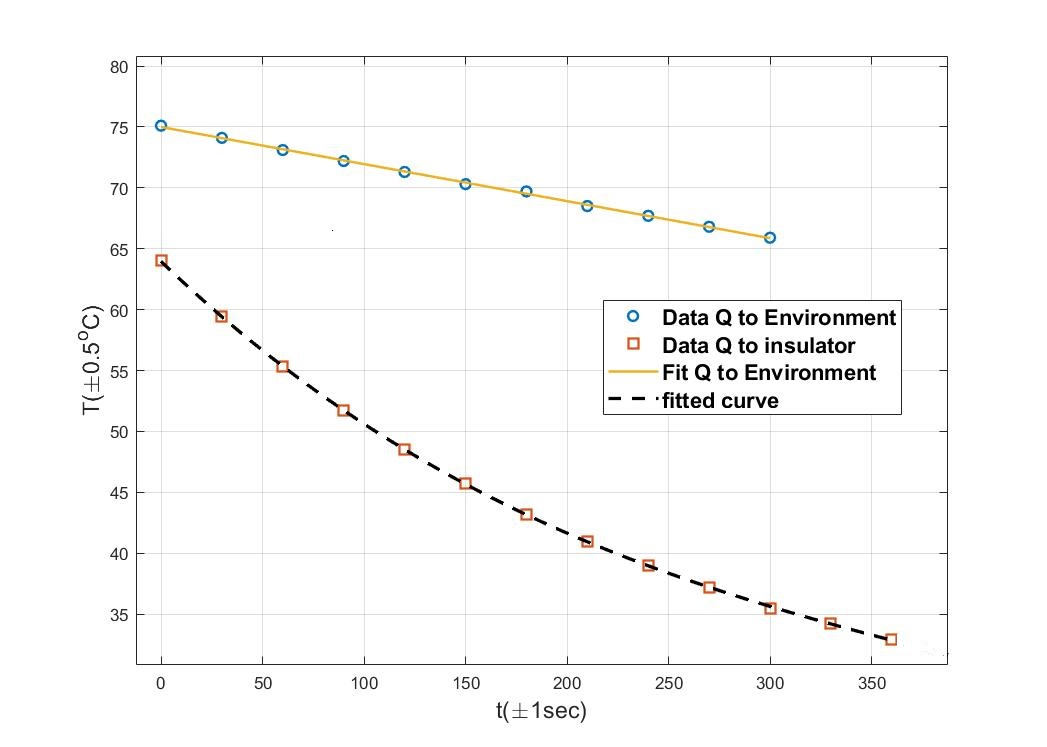
\includegraphics[scale=0.75]{insulator_heat.jpg}
\end{figure}

Από την σχέση (\ref{7}) έχουμε ότι 
\begin{align*}
ln(T-T_\pi') = ln(T_0- T_\pi') - \frac{\lambda S}{mca} t
\end{align*}
Έτσι, αν θεωρήσουμε $Y=ln(T-T_\pi')$, $X = t$, $A=ln(T_0-T_\pi')$ και $B=-\frac{\lambda S}{mca}$, προκύπτει η ευθεία $Y=A+BX$, για την οποία έχουμε μετρήσει πειραματικά τα $Y,X$. Πάλι με την γραφική μέθοδο μπορούμε να προσδιορίσουμε τα $A,B$, ωστόσο θα περιοριστούμε μόνο στην κλίση, καθώς σε αυτήν περιέχεται ο συντελεστής θερμικής αγωγιμότητας του μονωτή που μας ενδιαφέρει. Η κύρια ευθεία καθώς και οι δύο καλύτερες που περνάνε από τα σημεία κάτω και πάνω από αυτήν φαίνονται στην Εικόνα 6.


%%%%%%%%%%%%%%%%% UP %%%%%%%%%%%%%%%%%%%%%%%%%%%%%
%\begin{figure}[h!]
%\centering 
%\caption{ Ευθεία κλίσης $B=-\frac{\lambda S}{mca}$}
%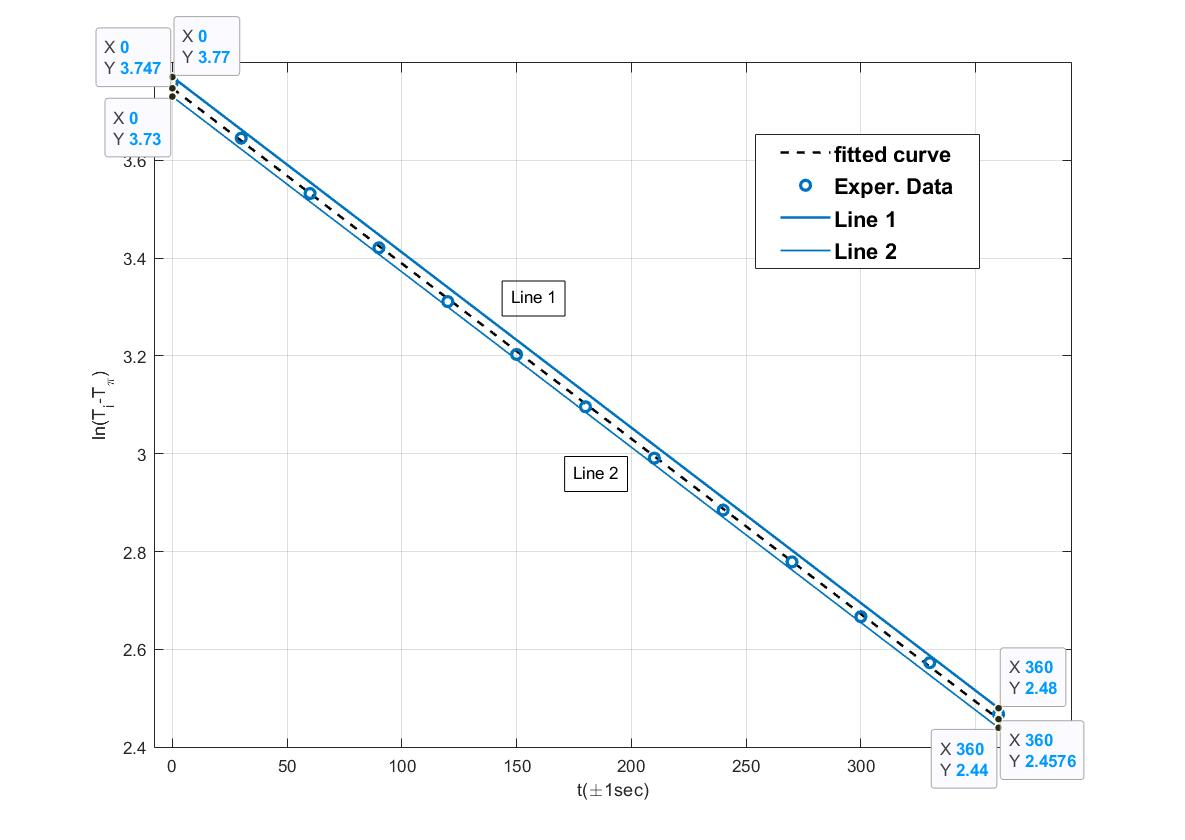
\includegraphics[scale=0.4]{insulator_1_up.jpg}
%\end{figure}
%
%Η κλίση της κύριας ευθείας είναι 
%\begin{align*}
%B = \frac{2.46-3.75}{360} = -0.00358
%\end{align*}
%ενώ αντίστοιχα οι κλίσεις των καλύτερων ευθειών 1,2 όπως προκύπτουν από την γραφική είναι
%\begin{align*}
%B_1= \frac{2.48-3.77}{360}=-0.0036    \text{ και  } B_2 = \frac{}{}
%\end{align*}
%Το σφάλμα της κλίσης της κύριας ευθείας που μας ενδιαφέρει είναι: 
%\begin{align*}
%\delta B = 0.5(B_2-B_1)  = 
%\end{align*}
% Άρα θα έχουμε $B=(\pm) [S.I.]$. Επομένως, γνωρίζοντας ότι 
%\begin{align*} 
%B=-\frac{\lambda S}{mca} \Rightarrow \lambda_{insul.} = - \frac{mcaB}{S}
%\end{align*}
%Το αντίστοιχο σφάλμα προκύπτει από την διάδοση των σφαλμάτων των m, B, aκ ιαι S: 
%\begin{align*}
%\delta \lambda_{insul.} = \sqrt{\left(\pdv{\lambda_{insul.}}{m} \delta m \right)^2+ 
%			\left( \pdv{\lambda_{insul.}}{a} \delta a\right)^2 + \left( \pdv{\lambda_{insul.}}{B} \delta B\right)^2+ \left( \pdv{\lambda_{insul.}}{S} \delta S\right)^2} 
%\end{align*}



%%%%%%%%%%%%%% CROSS %%%%%%%%%%%%%%%%%%%%%%%%
\begin{figure}[h!]
\centering 
\caption{ Ευθεία κλίσης $B=-\frac{\lambda S}{mca}$}
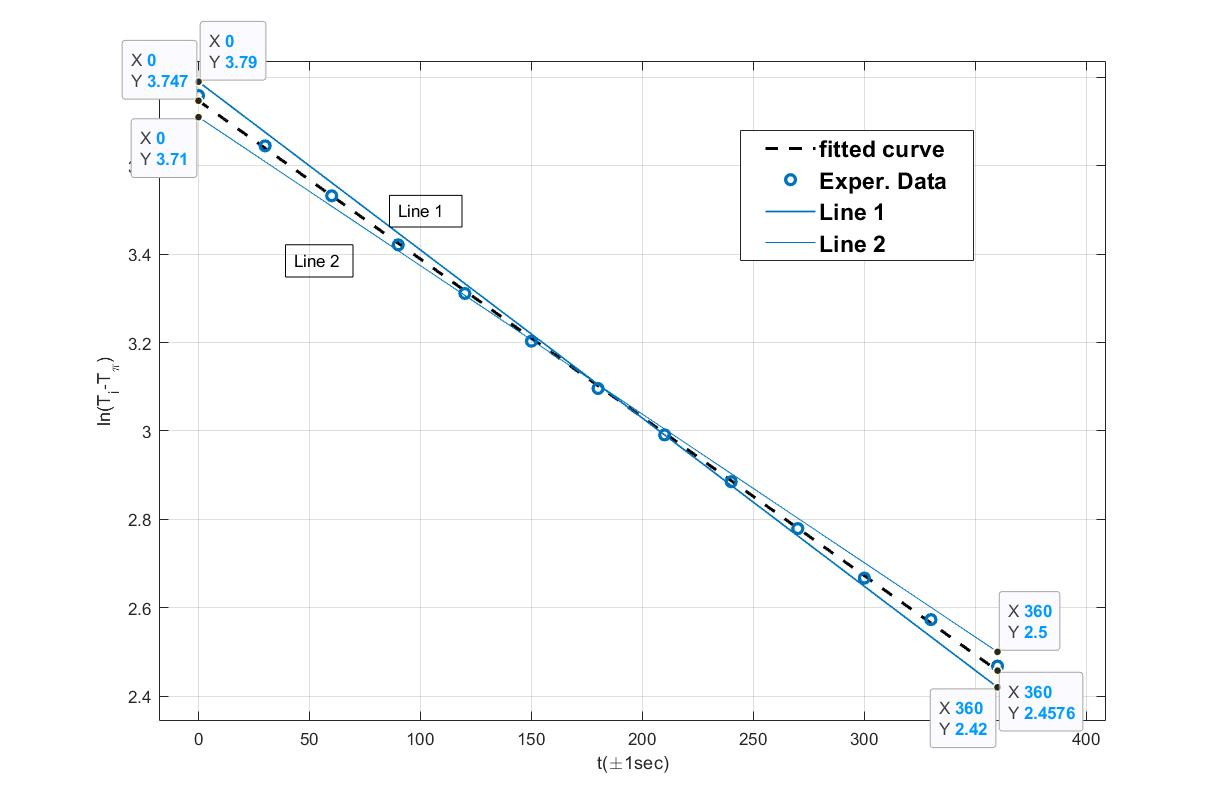
\includegraphics[scale=0.4]{insulator_1_cross.jpg}
\end{figure}
\textcolor{white}{g}  \newline\newline
Η κλίση της κύριας ευθείας είναι 
\begin{align*}
B = \frac{2.46-3.75}{360} = -0.0036 = -3.6\times10^{-3}
\end{align*}
ενώ αντίστοιχα οι κλίσεις των καλύτερων ευθειών 1,2 όπως προκύπτουν από την γραφική είναι
\begin{align*}
B_1= \frac{2.42-3.79}{360}=-0.0038=-3.8\times10^{-3}    \text{ και  } B_2 = \frac{2.50-3.71}{360}=-0.0033 = -3.3\times10^{-3}
\end{align*}
Το σφάλμα της κλίσης της κύριας ευθείας που μας ενδιαφέρει είναι: 
\begin{align*}
\delta B = 0.5(B_1-B_2)  = 0.00025 \simeq 0.3\times10^{-3}
\end{align*}
 Άρα θα έχουμε $B=(3.6\pm0.3)\times10^{-3} [S.I.]$. Επομένως, γνωρίζουμε ότι
 \footnote{Η ειδική θερμότητα του ορείχαλκου είναι $c=370Jkg^{-1}K^{-1}$ και το εμβαδό του δίσκου $S=\pi(d_2/2)^2 = 2.7\times10^{-3}m^2$ με σφάλμα από διάδοση $\delta S = \pdv{S}{d_2}\delta d_2 = \pi d_2(\delta d_2)/2  \stackrel{\text{$\delta d_2 =0.3mm$}}{=} 0.0028\times10^{-3}\simeq 0.1\times10^{-3}  m^2$}
 
\begin{align*} 
B=-\frac{\lambda S}{mca} \Rightarrow \lambda_{insul.} = - \frac{mcaB}{S} = 0.731 \simeq 0.73      [S.I.]
\end{align*}
Το αντίστοιχο σφάλμα προκύπτει από την διάδοση των σφαλμάτων των m, B, a και S: 
\begin{align*}
\delta \lambda_{insul.} = \sqrt{\left(\pdv{\lambda_{insul.}}{m} \delta m \right)^2+ 
			\left( \pdv{\lambda_{insul.}}{a} \delta a\right)^2 + \left( \pdv{\lambda_{insul.}}{B} \delta B\right)^2+ \left( \pdv{\lambda_{insul.}}{S} \delta S\right)^2} 
\end{align*}
Όμως επειδή τα σχετικά σφάλματα των m, S είναι $\sim 0.03\%, 0.1\%$ αντίστοιχα, δηλαδή είναι πολύ μικρά σε σχέση με των a, B που είναι $\sim 5\%, 8\%$, δεν θα συνεισφέρουν πολύ στο ολικό σφάλμα, άρα τα αγνοούμε και γίνεται
\begin{align*}
\delta \lambda_{insul.} =  \sqrt{ \left( \pdv{\lambda_{insul.}}{a} \delta a\right)^2 + \left( \pdv{\lambda_{insul.}}{B} \delta B								\right)^2}  = 
\frac{mc}{S}\sqrt{\left( B\delta a\right)^2 + \left( a \delta B\right)^2}	\simeq 	 0.07 
\end{align*}
Άρα για τον μονωτή έχουμε $\boxed{\lambda_{insul.}=(0.73\pm0.07)WK^{-1}m^{-1}}$.

\subsection*{Συμπεράσματα}
Πρέπει να παρατηρήσουμε ότι η μία εκ των δύο αρχικών παραδοχών για τις συνοριακές συνθήκες, δηλαδή ότι η θερμοκρασία του ενός άκρου είναι ίση με εκείνη του περιβάλλοντος, άρα σταθερή, καταρρέει καθώς η θερμοκρασία του περιβάλλοντος μετρήθηκε διαφορετική στην αρχή και στο τέλος του πειράματος με μεταβολή 2.3$^oC$. Αυτό σε πρώτη ματία, ίσως να μπορεί να θεωρηθεί ως μία παράμετρος που επηρέασε τις αριθμητικές τιμές των συντελεστών. 
Ωστόσο, στο κάθε μέρος χρησιμοποιήσαμε την θερμοκρασία που μετρήσαμε πιο κοντά σε αυτό (1o μερος $->$ Αρχική θερμοκρ. $\&$ 2ο μέρος $->$ Τελική θερμοκρ.). Έτσι, αν συνυπολογίσουμε το γεγονός ότι η μεταβολή αυτή αναφέρεται σε όλη τη διάρκεια του πειράματος, συνεπώς κατά το πέρας του 1ου μέρους θα ήταν ακόμη πιο μικρή και αντίστοιχα για το δεύτερο, θα μπορούσαμε να πούμε ότι η $\Delta T$ σε κάθε μέρος ήταν της τάξης του $1^oC$, ακόμη μικρότερη από την συνολική. Έτσι, ενδεχομένως να μην έχει και πολύ μεγάλη επίδραση στις μετρήσεις.

Ακόμη, επιβεβαιώνονται τα θεωρητικώς αναμενόμενα ότι δηλαδή $\lambda_{cond.}>\lambda_{insul.}$, ότι η θερμοκρασία της ράβδου έχει γραμμική κατανομή στην μόνιμη κατάσταση ισορροπίας και και ότι η απώλεια θερμότητας του δίσκου προς το περιβάλλον είναι πολύ μικρή (γραμμική μείωση) σε σχέση με την απώλεια όταν έρχεται σε επαφή με τον μονωτή (εκθετική μείωση).
\subsection*{Βιβλιογραφία}
\begin{itemize}
\item[.] ΕΡΓΑΣΤΗΡΙΑΚΕΣ ΑΣΚΗΣΕΙς ΦΥΣΙΚΗΣ ΤΟΜΟΣ ΙΙ, ΣΥΛΛΟΓΙΚΟ
\end{itemize}

\end{document}